\section{Time Projection Chamber (TPC)}

	Στο αμέσως επόμενο στρώμα απο τον FTPC υπάρχει ένας τυπικός TPC (αυτός είναι και ο βασικός ανιχνευτής του STAR), που ανακατασκευάζει την τρισδιάστατη τροχιά των φορτισμένων σωματιδίων που παράγονται από τα γεγονότα κρούσεων στον RHIC. 
	Σε μία κεντρική κρούση Au-Au παράγονται περίπου 1000 πρωτογενή σωματίδια τα οποία με την σειρά τους αλληλεπιδρούν με το αέριο στο εσωτερικό του TPC και γεννούν  δευτερογενή σωματίδια. 
	Ο TPC μπορεί να ταυτοποιήσει τα δευτερογενή, αλλά και να ανακατσκευάσει περίπου 3000 από τις τροχιές τους, που ενδεχομένως θα οδηγήσουν σε συμπεράσματα για την αρχική κρούση. Μπορεί να ανακασκευάσει τροχιές από σωματίδια με μέση ορμή $100MeV/c<\braket{p}<1GeV/c$ και να μετρήσει την ορμή σωματιδίων με $100MeV/c<\braket{p}<30GeV/c$.
	
	Γεωμετρικά, πρόκειται για έναν κυλινδρικό θάλαμο με μήκος 4.2m και ακτίνας 4m ο οποίος περιέχει ένα μίγμα αερίων και είναι τοποθετημένος στο εσωτερικό ενός σωληνοειδούς με μαγνητικό πεδίο εως 0.5Τ. Επίσης, το εσωτερικό του χωρίζεται στα δύο από μία λεπτή μεμβράνη σε υψηλή τάση μεταξύ της οποίας και των άκρων επιβάλλουμε ηλεκτρικό πεδίο της τάξης των $~135V/cm$.
	
\begin{figure}[h!]
    \centering
    \subfloat[\centering Γεωμετρία]{{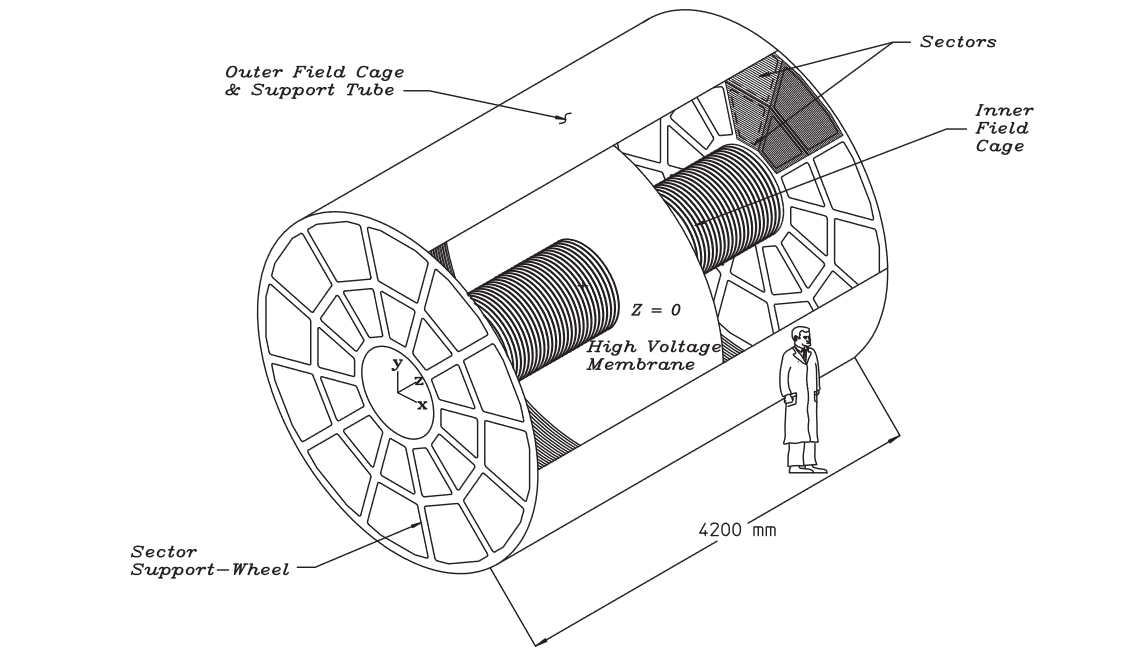
\includegraphics[scale=0.35]{STAR_Detectors/STAR_TPC} }}%
    \qquad
    \subfloat[\centering Φωτογραφία από το εσωτερικό]{{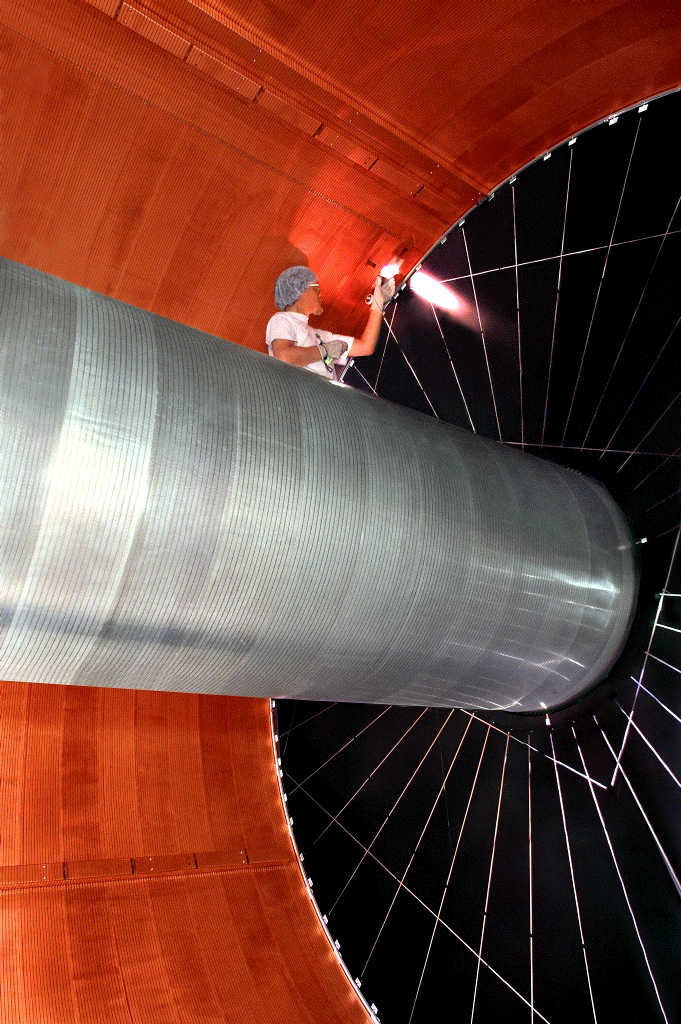
\includegraphics[width=4.5cm]{STAR_Detectors/InsideTpc} }}%
    \caption{O TPC }%
    \label{fig3.6}%
\end{figure}					
	 
	 Η τροχιά των σωματιδίων που ανιχνεύονται και χρησιμοποιούνται στην ανακατασκευή εξαρτάται από το ηλεκτρικό πεδίο. Άρα, δεδομένου ότι αυτά ταξιδεύουν έως και 2.1m, μία μικρή εκτροπή τους, που να οφείλεται σε ανομοιογένεια του πεδίου, μπορεί να οδηγήσει σε μεγάλη αλλοίωση της τροχιάς και κατ' επέκταση σε κακή ανακασκευή.
	Επομένως, η ομογένεια του ηλεκτρικού πεδίου είναι κρίσιμη καθώς η ανακατασκευή των τροχιών πρέπει γίνεται με ακρίβεια καλύτερη του χιλιοστού.
	
	Εξαιτίας του ηλεκτρικού πεδίου, τα δευτερογενή ηλεκτρόνια που παράγονται ολισθαίνουν προς τις βάσεις του κυλίνδρου όπου και ανιχνεύονται από το Σύστημα Ανάγνωσης (Readout System). 
	Αυτό βασίζεται σε Multiwire Proportional Chambers (MWPC) με Readout Pads. Oι MWPC έχουν συρμάτινες ανόδους ακτίνας 20μm που παρέχουν ενίσχυση σήματος. Το επαγόμενο φορτίο από μία χιονοστιβάδα μοιράζεται σε πολλά γειτονικά \textcolor{red}{pads} για ακριβέστερη ανακατασκευή.  Συνολικά υπάρχουν 136.608 pads.
	
	Το αέριο εντός του TPC είναι συνήθως μίγμα 10\%μεθανίου - 90\% Αργού σε πίεση 2mbar μεγαλύτερη της ατμοσφαιρικής. Ένα βασικό του χαρακτηριστικό είναι το ότι έχει τυπική ταχύτητα ολίσθησης που μεγιστοποιείται σε μικρές τιμές ηλεκτρικού πεδίου.
	
	Η διακριτική ικανότητα της θέσης καθορίζεται από την διάχυση των δευτερογενών ηλεκτρονίων ενώ η δυνατότητα ανίχνευσης σωματιδίων, που βασίζεται στην απώλεια ενέργειας, περιορίζεται από τις διακυμάνσεις στον ιονισμό και το πεπερασμένο μέγεθος του θαλάμου καθώς πολλά από αυτά δεν θα προλάβουν να εναποθέσουν όλη τους την ενέργεια.
	
\subsection{Μίγμα Αερίων}
	Ας ξεκινήσουμε από τα πιό απλά, ή τουλάχιστον αυτά που θα παρουσιαστούν ως πιό απλά σε αυτή την εργασία. Τα μίγματα αερίων που χρησιμοποιούνται είναι το 10\%μεθανίου - 90\% Αργού και το 50\%He+50\% $C_2H_6$. Τα εν λόγω αέρια επιλέχθηκαν με κριτήρια όπως η καθαρότητα που μπορεί να επιτευγχθεί, η εύκολη διατήρησή της, η ταχύτητα ολίσθησης, το κόστος, η ασφάλεια.
	
	Τα αέρια, συνολικού όγκου 50.000lt, κυκλοφορούν σε ένα κλειστό σύστημα με ροή 36.000lt/hr, όπου διαρκώς φιλτράρονται και απομακρύνται τα ξένα στοιχεια. Για παράδειγμα, αν έχουμε στοιχεία υψηλής ηλεκτραρνητικότητας τότε αυτά θα επιβραδύνουν τα δευτερογενή ηλεκτρόνια που θέλουμε να ανιχνεύσουμε, αλλοιώνοντας τα σήματά μας. Έτσι, είναι αναγκαίο το να κρατάμε τα επίπεδα οξυγόνου και νερού κάτω από 100ppm και 10ppm  αντίστοιχα. 	
	
	Χαρακτηριστικά του αερίου χρησιμοποιούνται επίσης για τον σχεδιασμό άλλων σημείων του TPC. Ενδεικτικά, αν ένα σωματίδιο ταξιδέψει όλο το δυνατό μήκος των 2.10m τότε η κάθετη διάχυση είναι $\sigma_T=3.3mm$ και αυτό μας καθορίζει την κλίμακα του συστήματος ανάγνωσης στα άκρα του TPC.
	% ενώ η διαμήκης $\sigma_L=5.2mm$ η οποία για ταχύτητα ολίσθησης 5.45cm/μs αντιστοιχεί σε χρόνο 230ns. 

	
	Η ταχύτητα ολίσθησης στο αέριο μεθανίου -  Αργού συναρτήσει του λόγου του πεδίου προς την πίεση για διάφορες τιμές συγκεντρώσεων φαίνεται στην Εικόνα (\ref{fig3.7}). Είναι λογικό να επιλέξουμε πεδίο τέτοιο, ώστε να είναι κοντά στο μέγιστο των καμπυλών. Αυτό, προκειμένου να εξασφαλίσυομε ότι η ταχύτηα θα είναι όσο λιγότερο ευαίσθητη σε μικροαλλαγές πίεσης και πεδίου. Παρ' όλα αυτά, επειδή στον TPC του STAR υπάρχει ένα σύστημα αυτόματου ελέγχου της ταχύτηας ολίσθησης που μετρά την αντίστοιχη ταχύτητα σωματιδίων που προέρχονται από ιονισμό μέσω Laser, γίνονται αυτόματες μικροδιορθώσεις στο ηλεκτρικό πεδίο για να εξισορροπηθούν οι μεταβολές της λόγω πίεσης. Επομένως, δεν θα πρέπει να υπάρχει η μέγιστη ταχύτητα, αλλά λίγο μικρότερη. Αυτό είναι αναγκαίο για την λειτουργία του συστήματος αυτόματου ελέγχου καθώς αν λειτουργούσαμε με την μέγιστη και εκείνο μετρούσε μία μείωσή της δεν θα ήταν ικανό να καθορίσει προς τα ποιά μεριά της καμπύλης συνέβη η μείωση, άρα δεν θα μπορούσε να καθορίσει κατάλληλα την αλλαγή στο πεδίο.
	
	%\begin{figure}[h!]
	%	\centering 
	%	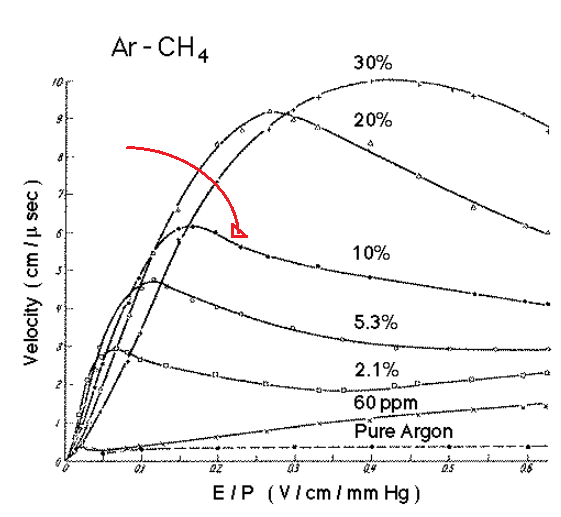
\includegraphics[scale=0.45]{STAR_Detectors/Gases}
	%\caption{Συνάρτηση της ταχύτητας ολίσθησης ως προς τον λόγο πεδίου/Πίεση }
	%	\label{fig3.7}
	%\end{figure}
	\begin{figure}[h!]
		\centering
		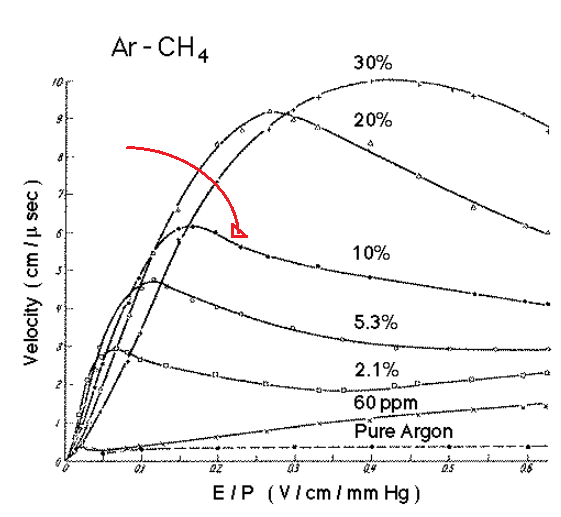
\includegraphics[scale=0.45]{STAR_Detectors/Gases}
   	\caption{Συνάρτηση της ταχύτητας ολίσθησης ως προς τον λόγο πεδίου/Πίεση }
		\label{fig3.7}
	\end{figure}	
	
\subsection{ Field Cage (Κυλινδρικό Κέλυφος)  }
	Tώρα θα ασχοληθούμε με τα γεωμετρικά όρια του TPC, τα οποία καθορίζουν τα χαρακτηριστικά του. Θα ξεκινήσουμε από αυτά που δεν περιλαμβάνουν τις συσκευές ανίχνευσης, δηλαδή με το κυλινδρικό κέλυφος και την εσωτερική άνοδο και στην συνέχεια θα ασχοληθούμε με τις βάσεις. Το σύστημα όλων των τοιχωμάτων επιβάλλει τις συνοριακές συνθήκες για το ομογενές ηλεκτρικό πεδίο, επομένως είναι σημαντικό να τοποθετηθούν με ακρίβεια. Για παράδειγμα η κεντρική μεμβράνη θα πρέπει να είναι ακριβώς παράλληλη με τις βάσεις.
	
	Αρχικά, σχετικά με την κεντρική μεμβράνη (Cenral Membrane - CM ). Αυτη πρόκειται για έναν κυκλικό φλοιό 70$\mu m$ από άνθρακα με επίστρωση από το πολυμερές Kapton, έχει μία εσωτερική οπή για να εφαρμόζει στον εσωτερικό κύλινδρο, και  της  εφαρμόζουμε δυναμικό 28kV σε αντίθεση με τις βάσεις που είναι γειωμένες. Άρα η CM είναι η ανοδος. Όμως, όπως έχει αναφερθεί, θέλουμε τον ακριβή προσδιορισμό του πεδίου στο εσωτερικό του TPC, υπάρχουν τοποθετημένες σε κάθε πλευράς της μεμβράνης 36 λωρίδες αλουμινίου. Το αλουμίνιο είναι ένα υλικό με χαμηλό έργο εξόδου. Έτσι, αν το στοχεύσουμε με UV-Laser θα προκαλέσουμε την εξαγωγή ηλεκτρονίων από αυτό. Μετρώντας αυτά τα ηλεκτρόνια μπορεί να γίνει η βαθμονόμηση του συστήματος προσδιορίζοντας ακριβώς τις θέσεις των λωρίδων αλουμινίου άρα των ορίων του θαλάμου και κατ' επέκταση τις μεταβολές στο πεδίο.
	
	Ο εσωτερικός και ο εξωτερικός κύλινδρος εξυπηρετούν δύο σκοπούς,  περιορίζουν το αερίο και θέτουν τις Συνοριακές Συνθήκες για το πεδίο. Η μηχανική τους σχεδίαση έγινε με στόχο την ελάττωση της μάζας και την μείωση των σκεδάσεων Coulomb στο εσωτερικό τους που αλλοιώνουν τις τροχιές. 
	Τα τοιχώματά τους δεν πρόκειται για απλά μεταλλικά υλικά αλλά για διαδοχικά στρώματα όπως φαίνεται στην Εικόνα (\ref{fig3.8}). 
	Πηγαίνοντας από έξω προς τα μέσα, η δομή έιναι Μεταλλικό στρώμα-Πολυμερές Kampton-Μεταλλικό στρώμα	
	Στο ενδιάμεσο αυτών υπάρχει το υλικό NOMEX σε σχήμα κυρηθρών το οποίο είναι ένα διηλεκτρικό, ελφρύ υλικό με μεγάλη αντοχή. 
	Κάθε 1.5mm υπάρχουν χαραγές προκειμένου να δημιουργηθούν ηλεκτρικά απομονωμένες περιοχές.
	% και να παρέχεται με ασφάλεια η τάση στα διαφορετικά δαχτυλίδια.
	 Η ελαχιστοποίηση της απόστασης των χαραγών στο 1.5mm είναι σημαντική τόσο για την μηχανική αντοχή, όσο και για την εκθεση του Kapton στο αέριο  η οποία μπορεί να αλλοιώσει το πεδίο εξαιτίας της τοπικής συγκέντρωσης φορτίων.
	
	
	\begin{figure}[h!]
			\centering 
			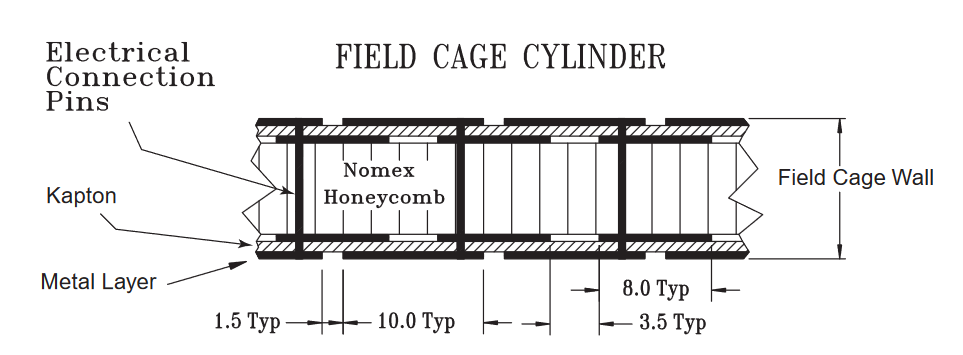
\includegraphics[scale=0.4]{STAR_Detectors/Inner_field_cage_wall}
			\caption{Το τοίχωμα του εσωτερικού φλοιού με διαστάσεις σε mm}
			\label{fig3.8}
		\end{figure}
		
	Ένα ακόμη σημαντικό σημείο είναι η ελαχιστοποίηση του υλικού στον εσωτερικό φλοιό καθώς εκεί λόγω της υψηλής πυκνότητας σωματιδίων είναι κρίσιμο να μειωθουν κατά το δυνατό οι αλληλεπιδράσεις Coulomb στο εσωτερικό του υλικού για την ακριβέστερη ανακατασκευή των τροχιών. 
	Στον εσωτερικό κύλινδρο, τα μεταλλικά κομμάτια είναι κατασκευασμένα από αλουμίνιο 12.8mm. με 0.5\% του radiation length $X_0$, ενώ στον εξωτερικό φλοιό, χάριν απλότητας, χρησιμοποιήθηκαν 10mm χαλκού σε 1.3\%$X_0$.
	
	Για την ηλεκτρική μόνωση των δύο φλοιών από τα γειτονικά τους κομμάτια χρησιμοποιούνται αέρια. Τα πλεονεκτήματα των αερίων έναντι των στερεών, είναι πως μειώνουν την δημιουργία δευτερογενών σωματιδίων σε αυτή την περιοχή όπου δεν μπορούν να ανιχνευτούν, ενώ ταυτόχρονα δεν υπάρχει η πιθανότητα για μόνιμη ζημία ή καταστροφή τους. Δηλαδή, μπορούν ανά πάσα στιγμή να ανανεωθούν χωρίς ιδιαίτερα υψηλό κόστος.
	
\subsection{End Caps (Βάσεις του Κελύφους)}

 Οι βάσεις είναι γειωμένες, με αποτέλεσμα το πεδίο στο δεξί και στο αριστερό μέρος του TPC  να είναι αντίθετο. 
 Σε αυτές είναι τοποθετημένοι οι  Mulitwire Proportional Chambers (MWPC) που πρόκειται για τους Readout Chambers που αποτελούν το πρώτο βήμα στην διαδικασία παραγωγής αξιοποιήσιμων σημάτων. Οι MWPC είναι αρθρωτοί θάλαμοι, δηλαδή διαφορετικές μονάδες που ενώνονται σε αλουμινένιες βάσεις. Η κυκλική βάση είναι χωρισμένη σε 12 τομείς που απέχουν 3mm μεταξύ τους και σε αυτούς είναι τοποθετημένοι οι εν λόγω θάλαμοι.  
	
	Ο κάθε MWPC αποτελείται από ένα επίπεδο pad και τρία επίπεδα από λεπτά σύρματα παράλληλα με το τοίχωμα (Εικόνα (\ref{fig3.9}). Το επίπεδο pad βρίσκεται στην εξωτερική πλευρά. Αμέσως δίπλα του υπάρχει το επίπεδο συρμάτων ανόδου, μετά τα \textcolor{red}{γειωμένα} σύρματα (σύρματα θωράκισης) και τέλος τα  σύρματα gating. Η κατεύθυνση των συρμάτων έχει επιλεγχθεί έτσι ώστε να βελτιστοποιείται η μέτρηση της ορμής των σωματιδίων με μέγιστη κάθετη ορμή $p_T$ των οποίων οι τροχιές είναι σχεδόν ευθείες που πηγάζουν από το σημείο κρούσης.
	%Είναι λοιπόν τοποθετημένα κάθετα στις τροχιές των σωματιδίων διότι τα σύρματα έχουν καλύτερη διακριτική ικανότητα κατά μήκος τους και όχι κατά την κατεύθυνση που διαχωρίζεται το ένα από το άλλο.
	Ομοίως, οι διαστάσεις των επίπεδων pad είναι τέτοιες, ώστε να βελτιστοποιείται η χωρική διακριτική ικανότητα των τροχιών. Πιό συγκεκριμένα, το κάθε pad έχει διαστάσεις ώστε το μεγαλύτερο μέρος φορτίου που δημιουργείται γύρω από μία άνοδο κατά μία χιονοστιβάδα Townsend να ανιχνεύεται μόνο από 3 pads. 
	
\begin{figure}[h!]
		\centering 
		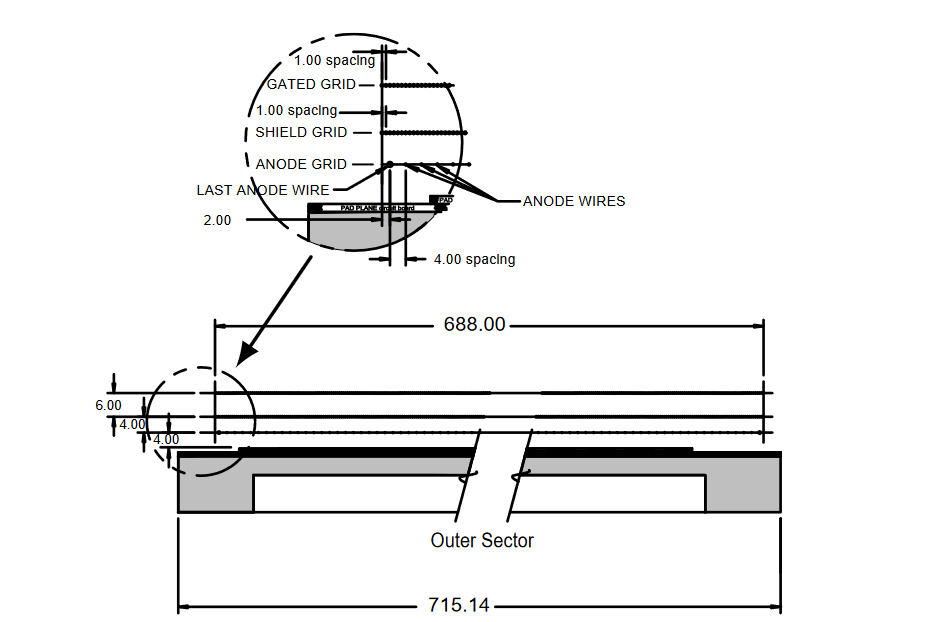
\includegraphics[scale=0.3]{STAR_Detectors/Readout_Sector}
		\caption{ Ένας MWPC του STAR του εξωτερικού τομέα. Οι διαστάσεις είναι σε mm.}
		\label{fig3.9}
	\end{figure}
		
	
	Υπάρχουν δύο υπό-τομείς με διαφορετική διαρρύθμιση των pads. Στον εξωτερικό, τα pads είναι πιό πυκνά για να δώσουν καλύτερη διακριτική ικανότητα στην απώλεια $dE/dx$, καθώς η μεγάλη πυκνότητα των pads εξασφαλίζει ανίχνευση και διάκριση μεγαλύτερου αριθμού σωματιδίων. H διαρρύθμιση εδώ είναι σε ένα τετραγωνικό πυκνό  πλέγμα. 
	Τα εσωτερικά pads είναι τοποθετημένα με διαφορετικό τρόπο. Εκεί, δεν μας ενδιαφέρει τόσο ο ακριβής προσδιορισμός της τροχιάς και της $dE/dX$, όσο το να διακρίνουμε δύο τροχιές. Η ελλάτωση των προσδοκιών εγκειται στο γεγονός ότι όντας κοντύτερα στα σημεία σύγκρουσης, η πυκνότητα των τροχιών είναι πολύ μεγαλύτερη άρα αυξάνεται η δυσκολία ανακατασκευής τους. Γι' αυτούς τους λόγους είναι τοποθετημένα σε διακριτές γραμμές .
	
	Μένει τώρα να ασχοληθούμε με τον σκοπό που εξυπηρετούν τα επίπεδα συρμάτων. 
Αρχικά, στην περιοχή γύρω από τα ανοδικά καλώδια, το ηλεκτρικό πεδίο επιταχύνει τα ηλεκτρόνια, αυξάνοντας το πλήθος τους μέσω Townsend, αφού υπάρχει επιπλέον ηλεκτρικό πεδίο μεταξύ αυτών και των pads που λειτουργούν ως κάθοδοι.
% αλλάζει κατεύθυνση και παύει να είναι παράλληλο με το μαγνητικό. Τότε ενισχύεται η ολίσθηση $\bm{E}\times\bm{B}$ και τα ηλεκτρόνια κινούνται προς τις ανόδους.
	Το πλέγμα θωράκισης έχει στόχο να περιορίζει το ηλεκτρικό πεδίο ανόδων-καθόδων εντός την περιοχής ενίσχυσης των ηλεκτρονίων. 
	Τέλος, το εξωτερικό πλέγμα, Gating Grid, λειτουργεί ως σύστημα ελέγχου των ηλεκτρονίων που εισέρχονται από τον θάλαμο ολίσθησης στον MWCP. Η τυπική του κατάσταση είναι να είναι "κλειστό" και να μην επιτρέπει την διέλευση των ηλεκτρονίων που έχουν παραχθεί από φορτισμένα σωματίδια στον θάλαμο ολίσθης.  Όταν όμως υπάρχει κάποιο ενδιαφέρον γεγονός, τότε "ανοίγει" και επιτρέπει την διέλευσή τους.
	
	Επίσης, στην περιοχή ενίσχυσης παράγεται μεγάλο πλήθος ιόντων που δημιουργούν μία χωρική κατανομή φορτίου η οποία αν περάσει στον κύριο θάλαμο ολίσθησης θα προκαλέσει ανεπιθύμητες διαταραχές στο ηλεκτρικό του πεδίο.  Έτσι,
ο δεύτερος σκοπός του gating grid είναι να εμποδίζει την διαφυγή των ιόντων. Όταν είναι σε "ανοιχτή" καταάσταση, τότε τα ιόντα λόγω μεγάλης μάζας, άρα μικρής ταχύτητας ολίσθης, δεν προφταίνουν να διαφύγουν, ενώ όταν είναι σε "κλειστή" κατάσταση παγιδεύονται από αυτό.
\vspace{-0.1cm}
\subsection{Η Επίδοση του TPC}
\subsubsection{Ανακατασκευή των x-y-z Θέσεων}
	H τροχιά ενός πρωτογενούς σωματιδίου ανακατασκευάζεται μέσω των συγκροτημάτων (clusters) δευτερογενών ηλεκτρονίων που ανιχνεύονται. Ο άξονας x ορίζεται ως ο άξονας που είναι παράλληλος στις σειρές των pads ενώ ο y επεκτέινεται από την δέσμη εως την μέση των σειρών με τα pads.
	Άρα για τον προσδιορισμό της x θέσης ψάχνουμε για ιονισμό κοντά σε γειτονικά pads της ίδια σειράς. Όταν δύο τροχιές συμπίπτουν μεταξύ τους, τότε τα pads θα ανιχνεύσουν ιονισμό που προέρχεται και από τις δύο. Ο διαχωρισμός τους γίνεται με κατάλληλους αλογρίθμους ενώ είναι αδύνατος ο προσδιορισμός της dE/dx. Περίπου το 30\% των τροχιών επικαλύπτωνται σε συγκρούσεις Au-Au 200GeV.
	Ο άξονας z ορίζεται ως ο άξονας που συμπίπτει με την δέσμη. Η z συντεταγμένη καθορίζεται από την μέτρηση του χρόνου ολίσθησης των cluster δευτερογενών ηλεκτρονίων. 
	%Ο χρόνος άφιξης των cluster υπολογίζεται μετρώντας τον χρόνο αφιξης των ηλεκτρονίνων σε ομάδες και παίρνωντας μέσο όρο.
	Έπειτα από την εύρεση των θέσεων του cluster των δευτερογενών ηλεκτρονίων, ένας αλγόριθμος ανακατασκευάζει όλη την τροχιά του σωματιδίου και έπειτα από αυτήν μπορούμε να εξάγουμε πληροφορίες για την ορμή του.

	Προφανώς, υπάρχουν διάφοροι παράγοντες που επιδεινώνουν την αρκίβεια προσδιορισμού της τροχιάς και οι οποίοι πρέπει να ληφθούν υπ' όψιν σε μετέπειτα διορθώσεις. Ενδεικτικά, μερικοί από αυτούς είναι η ανομοιογένεια το μαγνητικού πεδίου, η διαφορά στην γεωμετρία του εσωτερικού από του εξωτερικού τομέα με MWPC, η απόκλιση της καθόδου από την επιπεδότητα, η γωνιακή απόκλιση των \textbf{B, E} πεδίων και η συγκέντωση χωρικού φορτίου στον TPC. Οι παράγοντες αυτοί οδηγούν όλοι σε μία διόρθωση της θέσης της τάξης του 0.01cm.

\subsubsection{Ταυτοποίηση Σωματιδίων Μέσω της dE/dx}
	
	Η μέθοδος ταυτοποίησης των σωματιδίων μέσω της καμπύλης Bethe-Bloch λειτουργεί πιό αποδοτικά για σωματίδια με μικρή $p_T$ ορμή.  Όπως φαίνεται και στην Εικόνα (\ref{fig3.}), όσο μεγαλώνει η ορμή, τόσο μειώνεται η εξάρτηση της dE/dx από την μάζα του σωματιδίου. Άρα, η εναπόθεση ενέργειας είναι παρόμοια για όλα τα σωματίδια καθιστώντας αδύνατη την ανίχνευσή τους.
	
		Ο στόχος του STAR είναι η δυνατότητα για διάκριση μεταξύ Καονίων και πρωτονίων έως 1.2GeV/c κάτι που απαιτεί $\sigma_{dE/dx}$ διακριτική ικανότητα 7\%. Αυτή εξαρτάται από την ενίσχυση των φαινομένων Townsend άρα από την πίεση. Υπάρχει ένα σύστημα ελέγχου της πίεσης που μεριμνά για την διατήρηση της ενίσχυσης στα επιθυμητά επίπεδα. Ακόμη, μικρή επιδείνωση της διακριτικής ικανότητας προέρχεται από τις διαφορές των ηλεκτρονικών.
		Η καμπύλη dE/dx παράγεται από 45 συστοιχίες pad.
	
\begin{figure}[h!]
	\centering 
	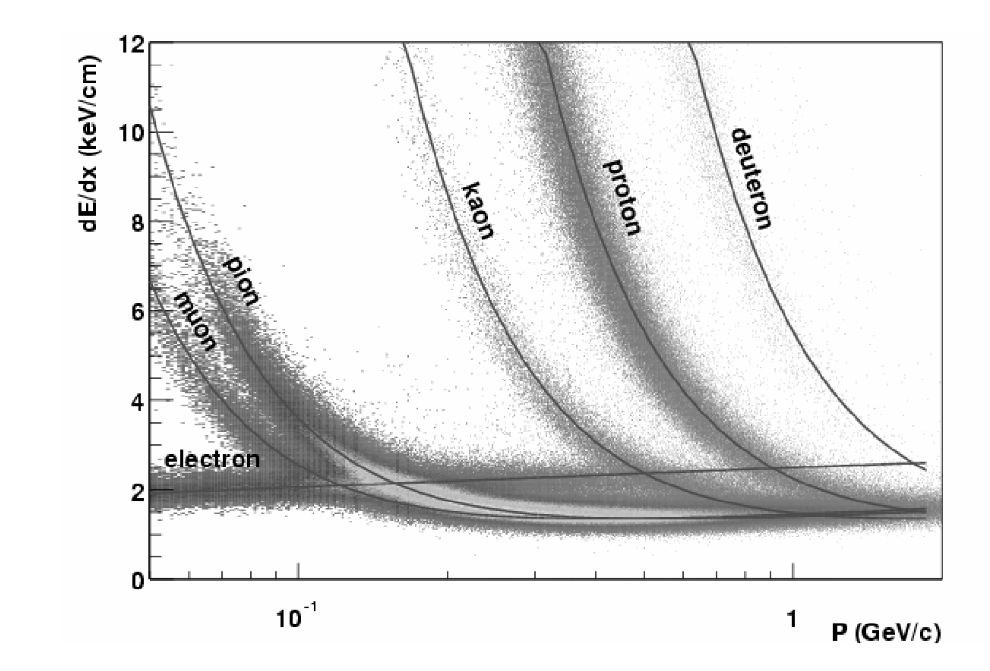
\includegraphics[scale=0.5]{STAR_Detectors/BB_Identification}
	\caption{Κατανομές απώλειας ενέργειας συναρτήσει της ορμής απ' τις οποίες γίνεται η ταυτοποίηση}
	\label{fig3.}
\end{figure}
